\documentclass[11pt]{article}
\usepackage{amssymb}
\usepackage{amsthm}
\usepackage{amsmath}
\usepackage{listings}
\usepackage{color}
\usepackage{graphicx}
\usepackage{gensymb}
\usepackage[margin=1.0in]{geometry}

\lstdefinestyle{matlab-style}{
language=Matlab,
basicstyle=\scriptsize\ttfamily,
tabsize=2,
rulecolor=,
language=matlab,
basicstyle=\scriptsize,
aboveskip={1.5\baselineskip},
columns=fullflexible,
showstringspaces=false,
extendedchars=true,
breaklines=true,
prebreak = \raisebox{0ex}[0ex][0ex]{\ensuremath{\hookleftarrow}},
frame=single,
showtabs=false,
showspaces=false,
showstringspaces=false,
identifierstyle=\ttfamily,
keywordstyle=\color[rgb]{0,0,1},
commentstyle=\color[rgb]{0.133,0.545,0.133},
stringstyle=\color[rgb]{0.627,0.126,0.941},
keepspaces=true,
numbers=left,
numbersep=5pt,
numberstyle=\tiny\color[rgb]{0.5,0.5,0.5},
stepnumber=1
}

\title{Design of an optimal heat exchanger\\MANE 6963 - Project 1}
\author{ID: 2168}
\date{}

\begin{document}

\maketitle

\section{Executive summary}

In this report, we investigate the optimal design of a heat exchanger that
heats air using hot water. An illustration of the geometry of the heat
exchanger is shown in Figure \ref{fig:exchanger}. The
goal of this investigation is to first define a geometry parameterization
$h = h(x, \boldsymbol{p})$ for the upper surface of the exchanger, where
$\boldsymbol{p} \in \mathbb{R}^{N_p}$ is the vector of design parameters
of length $N_p$. Then, using this geometry parameterization, we aim to
determine the parameter vector $\boldsymbol{p}$ that maximizes the heat
flux per unit length from the water to the air, $f(\boldsymbol{p})$.
\begin{figure}[htb]
\centering
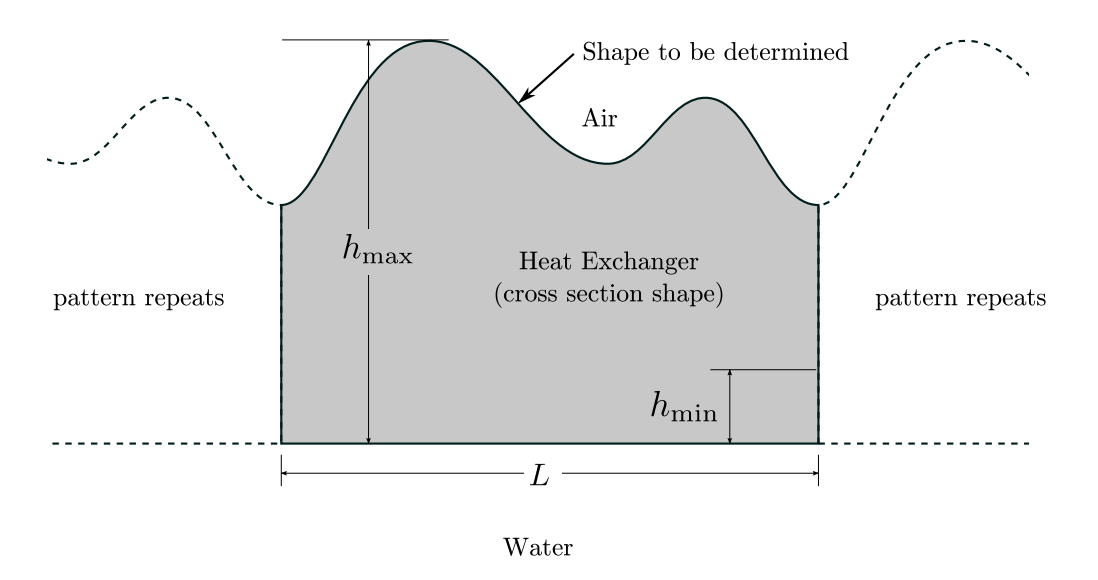
\includegraphics[scale=0.5]{exchanger}
\caption{Geometry of the heat exchanger design problem}
\label{fig:exchanger}
\end{figure}

To achieve this goal, we have:
\begin{itemize}
\item Defined an appropriate geometry parameterization
$h = h(x, \boldsymbol{p})$ of the upper surface of the exchanger.
\item Implemented a Matlab routine \textsc{SurfaceHeight.m} that
computes the parameterized surface height $h$.
\item Utilized a finite volume analysis method to approximate
the objective function $f(\boldsymbol{p})$ at a given fixed
geometry parameterization $h$.
\item Utilized Matlab's \textsc{fmincon} routine to determine an optimal
set of design parameters $\boldsymbol{p}$.
\item Performed a mesh convergence study using the optimized geometry
to ensure that the flux $f(\boldsymbol{p})$ is accurately computed.
\end{itemize}

The remainder of this report presents details of the theory and
implementations of the items in the list above. A listing of the
implemented Matlab routines is provided in the appendix.

\section{Geometry parameterization}

To parameterize the geometry of the top surface of the heat exchanger,
we have chosen a linear combination of the squares of trigonometric functions
of the form:
\begin{equation}
h(x, \boldsymbol{p}) = p_1 + \sum_{k=0}^{N_p} p_k
\left[ \sin \left( \frac{2 \pi (k-1) x} {L} \right) \right]^2
\end{equation}
We note that this form of parameterization supports
at most $2(N_p - 1)$ modes in the upper surface geometry. We choose
the number of design variables to be $N_p = 5$ to support a
relatively complex geometry while still maintaining computational
feasibility for the optimization routines. The Matlab routine
\textsc{SurfaceHeight.m} computes the surface height at discrete
spatial locations given an input design parameter vector
$\boldsymbol{p}$.

\section{Analysis methods}

To determine the flux per unit area from water to air, we first
approximate the temperature everywhere in the domain by solving the steady
state heat flux problem: find $T$ such that:
\begin{equation}
\begin{cases}
\begin{aligned}
\nabla \cdot ( \kappa \nabla T) &= 0, \quad x \in \Omega, \\
T(x,y=0) &= T_{\text{water}}, \\
T(x,h(x,\boldsymbol{p})) &= T_{\text{air}}, \\
T(x,y) &= T(x + L, y)
\end{aligned}
\end{cases}
\end{equation}
with a finite volume method. Here, $T$ is the temperature in the heat
exchanger domain $\Omega$, $\kappa$ is the thermal conductivity of the
heat exchanger, $T_{\text{air}}$ is the temperature in the air, and
$T_{\text{water}}$ is the temperature in the water. Dirichlet boundary
conditions are applied to the top and bottom surfaces of the domain,
while periodic boundary conditions are applied to the left and right
boundaries.

We assume that the temperature in the air $T_{\text{air}}$,
the temperature in the water $T_{\text{water}}$,
and the thermal conductivity $\kappa$ do not vary spatially.
To accurately account for the geometrical complexity of the upper
surface,
we choose a uniform grid of $N_x = N_y = 15*2(N_p-1)$
finite volumes in the $x$ and $y$ directions, so that the finest mode
of the geometry is resolved by at least $15$ finite volumes.
Once the temperature is computed everywhere in the domain,
the flux
\begin{equation}
f(\boldsymbol{p}) = \kappa \int_0^L
\frac{\partial T(x,y=0,h(x,\boldsymbol{p}))}{\partial y} \text{d} x
\end{equation}
from the air to the water is approximated with a first order
finite-difference scheme.

\section{Optimization problem statement}

Given the definitions of the surface height
$h(x, \boldsymbol{p})$ and the flux per unit area $f(\boldsymbol{p})$
from previous sections, the constrained optimization problem we wish
to solve is: 
\begin{equation}
\begin{aligned}
& \underset{\boldsymbol{p}}{\text{minimize}}
& & \left[ f(\boldsymbol{p}) \right]^{-1} \\
& \text{subject to}
& & h_{\text{min}} \leq h(x, \boldsymbol{p}) \leq h_{\text{max}}
\end{aligned}
\label{eq:optimize}
\end{equation}
Note that by minimizing the inverse of the flux, we are in fact maximizing
the flux. Here, we have constrained the surface height to be greater than
or equal to a minimum value $h_{\text{min}}$ and less than or equal
to a maximum value $h_{\text{max}}$. These constraints are
implemented in the routine \textsc{NonlinearConstraints.m} as
nonlinear constraints to be used in Matlab's  \textsc{fmincon} routine.

\section{Optimization methods}

We utilize Matlab's \textsc{fmincon} routine to solve the
optimization problem \eqref{eq:optimize}. By default, this routine performs
gradient-based optimization with a forward finite-difference approximation
of the gradient $\nabla f$. We provide \textsc{fmincon} with the
following options:
\begin{verbatim}
optns = optimoptions(@fmincon,...
     'Display','iter',...
     'Algorithm', 'sqp');
\end{verbatim}
Here we have chosen to use a sequentially quadratic programming
algorithm for the optimization routine, where we assume that the
objective function $f(\boldsymbol{p})$ is twice continuously
differentiable. We utilize \textsc{fmincon}'s default convergence
tolerances, as they are sufficiently accurate for our purposes.
The Matlab routine \textsc{MaxFluxDriver.m} solves
the optimization problem through a call to \textsc{fmincon}. Note
that we define the objective function $f = f(\boldsymbol{p})$ as
a function of the surface height $f = f(h(x, \boldsymbol{p}))$ on
line 26 of \textsc{MaxFluxDriver.m}.

\section{Results}

We choose the length of the analysis domain $L=0.05$m, the
number of design variables $N_p = 5$, the temperature of the
air to be $T_\text{water} = 90 \degree$ C, the temperature of the
water to be $T_\text{air} = 20 \degree$ C, the thermal
conductivity to be $\kappa = 20 W / (\text{m} \degree \text{C})$,
the minimum surface height to be $h_{\text{min}} = 0.01$m, and
the maximum surface height to be $h_{\text{max}} = 0.05$m.

The routine \textsc{MaxFluxDriver.m} was called with the defined
inputs:
\begin{verbatim}
>> p = MaxFluxDriver(L,Np,Tair,Twater,kappa,hmin,hmax);
\end{verbatim}
and returned the convergence history:
\begin{verbatim}
                                                          Norm of First-order
 Iter F-count            f(x) Feasibility  Steplength        step  optimality
    0       6    1.744341e-04   2.284e+00                           3.153e-04
    1      12    1.141534e-04   0.000e+00   1.000e+00   1.627e+00   9.419e-01
    2      18    1.135948e-04   0.000e+00   1.000e+00   7.350e-04   4.917e-04
    3      24    1.112710e-04   0.000e+00   1.000e+00   3.003e-03   6.215e-04
    4      30    1.056029e-04   0.000e+00   1.000e+00   7.910e-03   7.747e-04
    5      36    8.865227e-05   0.000e+00   1.000e+00   1.736e-02   1.642e-03
    6      42    5.429164e-05   1.919e-13   1.000e+00   2.298e-02   1.855e-03
    7      48    5.404953e-05   1.123e-14   1.000e+00   4.724e-04   4.259e-04
    8      54    5.249482e-05   0.000e+00   1.000e+00   2.535e-03   5.858e-04
    9      60    4.757424e-05   0.000e+00   1.000e+00   8.728e-03   6.114e-04
   10      66    4.246988e-05   1.735e-18   1.000e+00   8.774e-03   2.174e-04
   11      72    4.211768e-05   7.487e-15   1.000e+00   2.159e-03   1.940e-04
   12      78    4.049092e-05   1.735e-18   1.000e+00   9.320e-03   2.904e-04
   13      84    4.049092e-05   1.388e-17   1.000e+00   3.010e-12   6.811e-12
\end{verbatim}
where the optimal parameter vector $\boldsymbol{p}$ was found to be:

\newpage

\begin{verbatim}
p =

   0.010000000000000
  -0.000000000000000
   0.000000000000000
   0.000000000000000
   0.040441876010831
\end{verbatim}
The final geometry of the upper surface is shown in Figure
\ref{fig:geometry}. We note that only the highest order mode
$p_5$ contributes significantly to the complexity of the geometry
of the upper surface. This result is congruent with the engineering
intuition that the geometry that maximizes the flux will be the one with
the greatest surface area.

\begin{figure}[hbt]
\centering
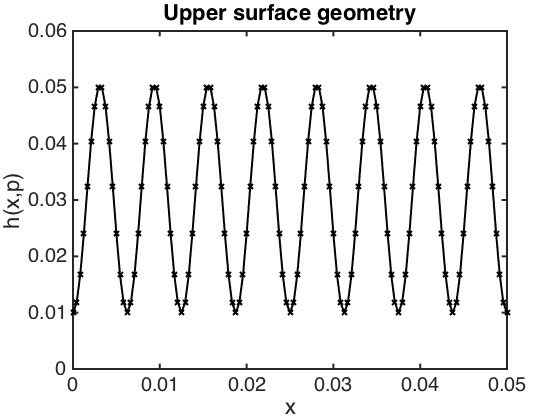
\includegraphics[width=0.5\textwidth]{geometry}
\caption{Final upper surface geometry}
\label{fig:geometry}
\end{figure}

\begin{figure}[hbt]
\centering
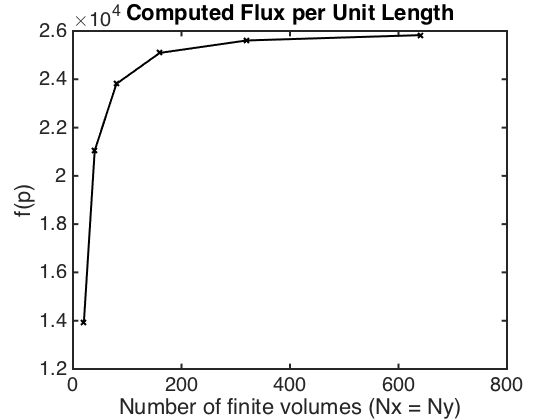
\includegraphics[width=0.5\textwidth]{flux}
\caption{Computed flux values at different grid spacings}
\label{fig:flux}
\end{figure}

The Matlab routine \textsc{ConvergenceDriver.m} was used to
perform a mesh convergence analysis on the optimal geometry
to ensure the accuracy of the computed flux value. The flux
was computed using uniform numbers $N_x = N_y = \{20,40,80,160,32,640\}$
of finite volumes in the $x$ and $y$ directions. The routine
\textsc{ConvergenceDriver.m} was called as:
\begin{verbatim}
>> n = [20,40,60,80,160,320,640]';
>> f = ConvergenceDriver(n,L,p,kappa,Tair,Twater);
\end{verbatim}
The computed flux values versus grid spacing are shown in Figure
\ref{fig:flux}. The relative percent difference between the flux
evaluated with $320$x$320$ volumes and $640$x$640$ volumes
is around $0.9\%$. Thus, we conclude that the flux value computed
with $640$x$640$ volumes is accurate enough for our purposes.
The computed flux value at this fine grid spacing is
\begin{equation}
f = 25,827.93 \text{W}/(\text{m} \degree \text{C}),
\end{equation}
which is approximately a $260\%$ increase over the nominal value
of $7,000 \text{W}/(\text{m} \degree \text{C})$
for a heat exchanger with a flat surface at $h = 0.01$m.

\section{Conclusions}

We have determined the shape of a heat exchanger
that optimizes the  flux per unit area from one surface of the heat
exchanger to the other using the gradient-based
optimization capabilities of Matlab's \textsc{fmincon} routine.
The accuracy of the flux value for this optimized geometry was verified
with a mesh convergence study, and a $260\%$ increase over the nominal
value. The shape of the final geometry is consistent with the engineering
intuition that the maximal flux for the heat exchanger will occur
with the greatest surface surface area.

\newpage

\section{Appendix: code listings}

\lstinputlisting[
  style=matlab-style,
  caption=SurfaceHeight.m]{SurfaceHeight.m}

\newpage

\lstinputlisting[ 
  style=matlab-style,
  caption=NonlinearConstraints.m]{NonlinearConstraints.m}

\newpage

\lstinputlisting[
  style=matlab-style,
  caption=MaxFluxDriver.m]{MaxFluxDriver.m}

\newpage

\lstinputlisting[
  style=matlab-style,
  caption=ConvergenceDriver.m]{ConvergenceDriver.m}

\end{document}
